\documentclass{standalone}
\usepackage{standalone}

\begin{document}

\subsection{Vertical Edge Density}
The vertical {\it Sobel operator} (Equation \ref{eq:Sobel}) is used to calculated the edge density. 
\begin{equation} \label{eq:Sobel}
h =
  \begin{bmatrix}
    -1 & 0 & 1\\
    -2 & 0 & 2\\
    -1 & 0 & 1
  \end{bmatrix} 
\end{equation}

Which we could obtain by using $sobel$ function from OpenCV library:
\begin{lstlisting}[language=Python]
sobel = cv2.Sobel(img, cv2.CV_8UC1, 1, 0, ksize=3)
\end{lstlisting}

Next, we applied a low threshold value to the gradient image. In this case, we used an adaptive threshold technique called {\it Otsu’s Binarization} using an offset value of $85$, which we obtained empirically. Result is shown in Figure \ref{fig:SobelSample}
\begin{figure}
	\centering
	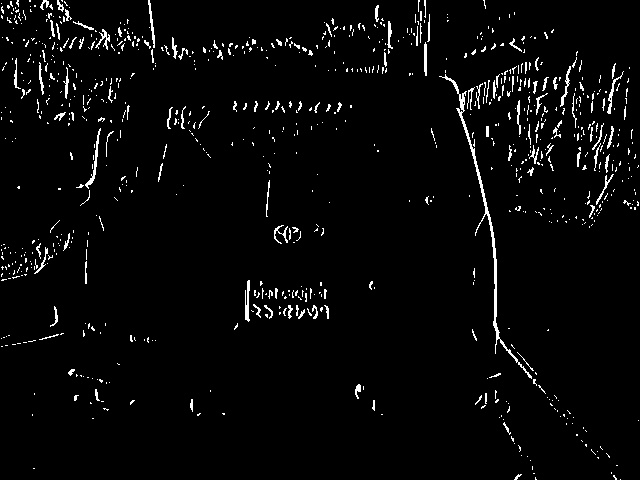
\includegraphics[width=.8\linewidth]{./img/sample/stage2.jpg}
	\caption{After applying Sobel Operator} 
	\label{fig:SobelSample}
\end{figure}

\end{document}